\documentclass{article}
\usepackage{tikz}
\usetikzlibrary{shapes,shadows,arrows}
\usepackage{pgfplots,pgfplotstable}
\pgfplotsset{compat=1.13}

\usepackage{fp}

\begin{document}
	
	\begin{figure}[ht]
		\centering
		\begin{center}
			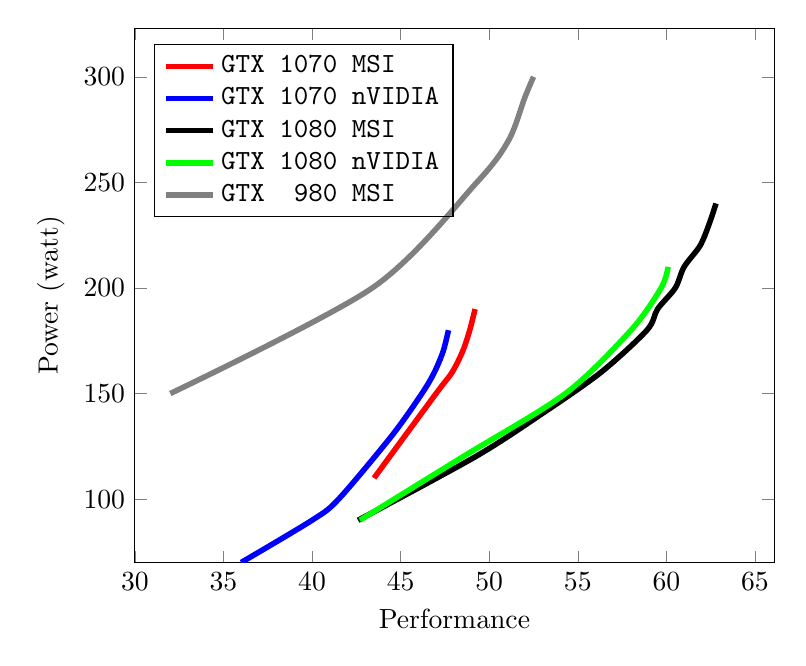
\begin{tikzpicture} %[>=latex]
			\begin{axis}[
			width=0.8\textwidth,
			%line width=2,
			%symbolic x coords={2012, 2013, 2014, 2015, 2016},
			%xticklabels={,,},
			%yticklabels={,,}
			%xticklabels={720p,1080p,4k},
			%minor xtick={0,1,...,18},
			grid=none,
			xmin=30,
			ymin=70,
			xlabel=Performance,
			ylabel=Power (watt),
			legend pos=north west,
			legend cell align=left,
			%legend columns=2, 
			legend style={
				fill=none,
			 	%/tikz/column 2/.style={
			 	%	column sep=5pt,
			 	%},
			 },
			%enlarge x limits=0.1,
			%xticklabel style={text width=0.2\textwidth,align=flush left},
			]
			\addplot[line width=2pt,smooth,color=red] coordinates {
				(43.5,110) (47,150) (47.9,160) (48.5,170) (48.9,180) (49.2,190)
			};
			\addplot[line width=2pt,smooth,color=blue] coordinates {
				(36,70) (40,90) (41.5,100) (44.5,130)
				(46.2,150) (46.9,160) (47.4,170) (47.7,180)
			};
			\addplot[line width=2pt,smooth,color=black] coordinates {
				(42.6,90) (49.2,120) (52.9,140) (56.3,160) (58.9,180) (59.5,190)
				(60.5,200) (61.0,210) (61.9,220) (62.4,230) (62.8,240)
			};
			\addplot[line width=2pt,smooth,color=green] coordinates {
				(42.7,90) (48.5,120) (54.3,150) (58.0,180) (59.7,200) (60.1,210)
			};
			\addplot[line width=2pt,smooth,color=gray] coordinates {
				(32.0,150) (43.4,200) (49.3,250) (51.1,270) (52.0,290) (52.5,300)
			};
			\legend{\texttt{GTX 1070 MSI}\\\texttt{GTX 1070 nVIDIA}\\\texttt{GTX 1080 MSI}\\\texttt{GTX 1080 nVIDIA}\\\texttt{GTX ~980 MSI}\\}
			%\draw[red] plot [smooth] coordinates {(0 0) (2,3700) (4,6006) (18,18000)};
			\end{axis}
			\end{tikzpicture}
		\end{center}
		\caption{Bandwidth required for delivering various videos.}\label{fig:bitrate-resolution}
	\end{figure}
	
\end{document}